% !TEX TS-program = pdflatex
% !TEX encoding = UTF-8 Unicode

% This is a simple template for a LaTeX document using the "article" class.
% See "book", "report", "letter" for other types of document.

\documentclass[11pt]{article} % use larger type; default would be 10pt

\usepackage[utf8]{inputenc} % set input encoding (not needed with XeLaTeX)

%%% PAGE DIMENSIONS
\usepackage{geometry} % to change the page dimensions
\geometry{a4paper} % or letterpaper (US) or a5paper or....

\usepackage{graphicx} % support the \includegraphics command and options

\usepackage{amssymb}
\usepackage{amsmath}
%%% PACKAGES
\usepackage{booktabs} % for much better looking tables
\usepackage{array} % for better arrays (eg matrices) in maths
\usepackage{paralist} % very flexible & customisable lists (eg. enumerate/itemize, etc.)
\usepackage{verbatim} % adds environment for commenting out blocks of text & for better verbatim
\usepackage{subfig} % make it possible to include more than one captioned figure/table in a single float
% These packages are all incorporated in the memoir class to one degree or another...

%%% HEADERS & FOOTERS
\usepackage{fancyhdr} % This should be set AFTER setting up the page geometry
\pagestyle{fancy} % options: empty , plain , fancy
\renewcommand{\headrulewidth}{0pt} % customise the layout...
\lhead{}\chead{}\rhead{}
\lfoot{}\cfoot{\thepage}\rfoot{}

%%% SECTION TITLE APPEARANCE
\usepackage{sectsty}
\allsectionsfont{\sffamily\mdseries\upshape} % (See the fntguide.pdf for font help)
% (This matches ConTeXt defaults)

%%% ToC (table of contents) APPEARANCE
\usepackage[nottoc,notlof,notlot]{tocbibind} % Put the bibliography in the ToC
\usepackage[titles,subfigure]{tocloft} % Alter the style of the Table of Contents
\renewcommand{\cftsecfont}{\rmfamily\mdseries\upshape}
\renewcommand{\cftsecpagefont}{\rmfamily\mdseries\upshape} % No bold!
\usepackage{graphicx}
\graphicspath{ {./pings/} }

\usepackage{amsmath}
\DeclareMathOperator*{\argmax}{arg\,max}
\DeclareMathOperator*{\argmin}{arg\,min}

\newcount\colveccount
\newcommand*\colvec[1]{
        \global\colveccount#1
        \begin{pmatrix}
        \colvecnext
}
\def\colvecnext#1{
        #1
        \global\advance\colveccount-1
        \ifnum\colveccount>0
                \\
                \expandafter\colvecnext
        \else
                \end{pmatrix}
        \fi
}

%%% END Article customizations

%%% The "real" document content comes below...

\title{Macro PS4}
\author{Michael B. Nattinger\footnote{I worked on this assignment with my study group: Alex von Hafften, Andrew Smith, and Ryan Mather. I have also discussed problem(s) with Emily Case, Sarah Bass, and Danny Edgel.}}

%\date{} % Activate to display a given date or no date (if empty),
         % otherwise the current date is printed 

\begin{document}
\maketitle
\section{Question 1}
\subsection{Part A}
We will solve for the equilibrium. 
Consumers maximize utility by choosing their asset savings (now the assets are, specifically, capital) subject to budget constraints.

Our bellman equation takes the following form:

\begin{align*}
V(k,l)&= \max_{k'} \frac{(wl + rk - k' + k(1-\delta))^{1-\gamma}}{1-\gamma} + \beta\sum_{i=1}^n(V(k',l_i)P(l'=l_i|l)
\end{align*}

Firms choose $N,K$ to maximize profits. We solve by taking first order conditions:
\begin{align*}
&\max_{w,r} K^{\alpha}N^{1-\alpha} - wN - rK\\
&\Rightarrow w = (1-\alpha)(K/N)^{\alpha},\\
&\Rightarrow r = \alpha(K/N)^{\alpha - 1}.
\end{align*}

We will proceed by solving the problem numerically. Note that labor supply is exogenous and, in the equilibrium, will always be 1. We do not know the equilibrium capital supply levels so we need to estimate this analytically. We will start at a guess for capital demand, calculate the model solution, and check to see if capital markets clear. We will use a nonlinear optimizer to minimize the deviation of capital supply and labor demand. Then, once the capital market clears, since we know that the labor market will also clear, Walras' law implies that the goods market will also clear.

The equilibrium levels of capital stock, wage, and the interest rate are as follows:


\begin{center}
\begin{tabular}{ll}
& Equilibrium \\ 
\hline 
Capital & 5.0451 \\ 
Wage & 1.1461 \\ 
Interest rate & 0.12778 \\ 
\hline 
\end{tabular}
\end{center}
\subsection{Part B}

We compare the consumption and income distributions by comparing their CDFs.

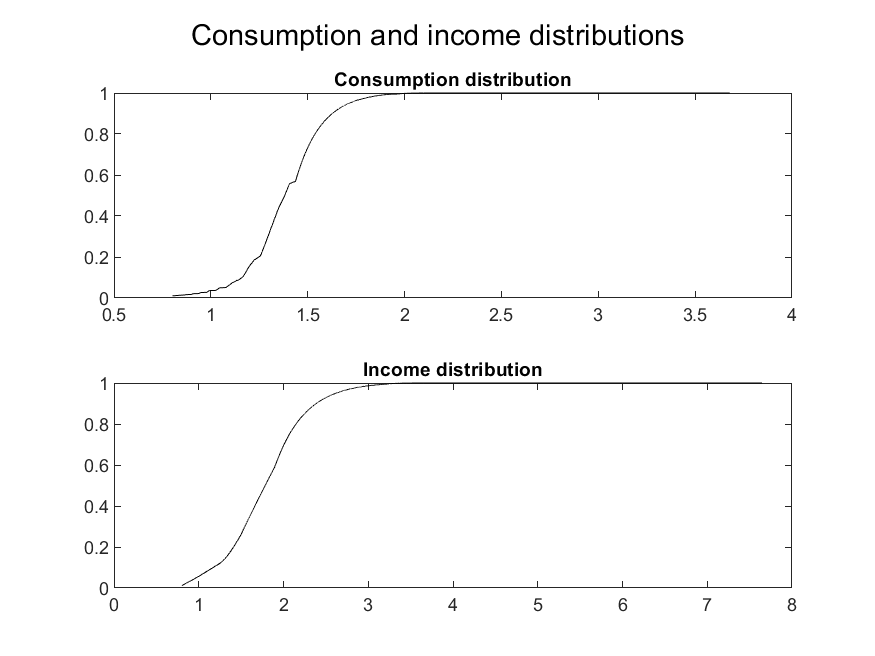
\includegraphics{dis}

Above we can see the distributions for consumption and income, as represented by their CDFs. The consumption distribution has a much tighter spread than the income distribution, with the vast majority of the population mass consuming between 1 and 1.7 units of the consumption good, while the majority of the population mass has an income between 1 and 2.5 units of the consumption good. This makes sense, as individuals make their asset savings choice to smooth consumption, so income spread should be wider than the consumption spread. Below, we will observe the change in the distribution from changing the lower bound on assets.

\subsection{Part C}

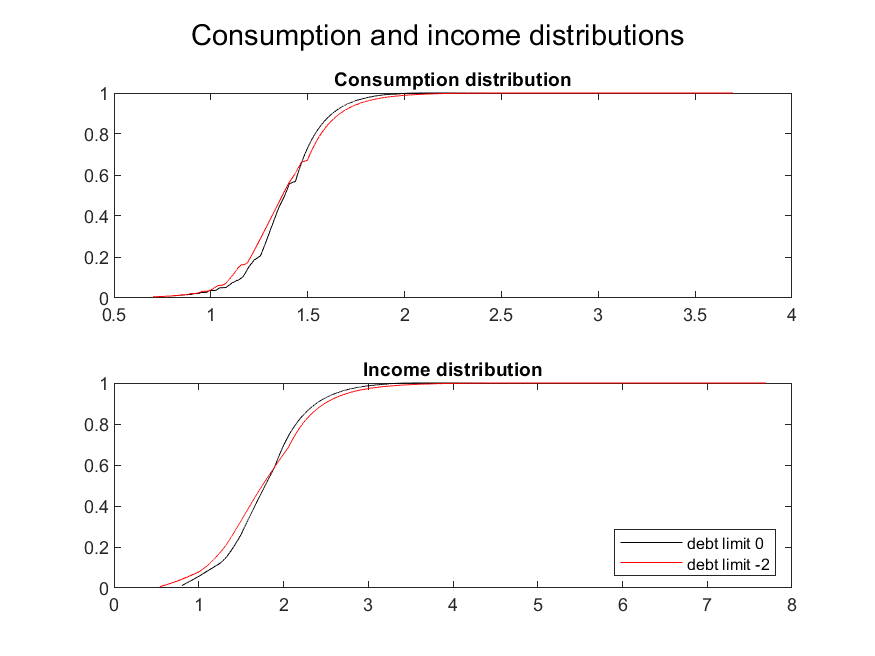
\includegraphics{comp}

With the lower debt limit, the consumption and income distributions widen. Individuals can get into debt, which they could not before, and if they are continually unlucky with respect to their labor draws, they will go into debt until they hit the lower bound, and if they hit the lower bound then they will be able to afford even less of the consumption good than before, should they continue to be unlucky in their draws. The result is a wider spread in both consumption and income. Below we compare the equilibrium variables in the debt equilibrium with those in Part A.

\begin{center}
R2 & 0.552 & 0.622 & 0.407 \\ 
N & 28 & 29 & 26 \\ 

\end{center}

We see, from the table above, that capital levels fall in the debt equilibrium. Further, the wage falls as labor is less productive with a lower capital level. Finally, the interest rate rises as the interest rate is determined by the derivative of output with respect to capital, which is decreasing in capital.

\section{Question 2}
\subsection{Part A}
Our bellman equation takes the following form:
\begin{align*}
V(k,z) &= \max_{k'} \frac{(zk^{0.35}+(1-\delta)k - k')^{1-\gamma}}{1-\gamma} + \beta\sum_{i=1}^n V(k',z_i)P(z' = z_i|z)
\end{align*}
 We solve this computationally, and compare to our results from before.

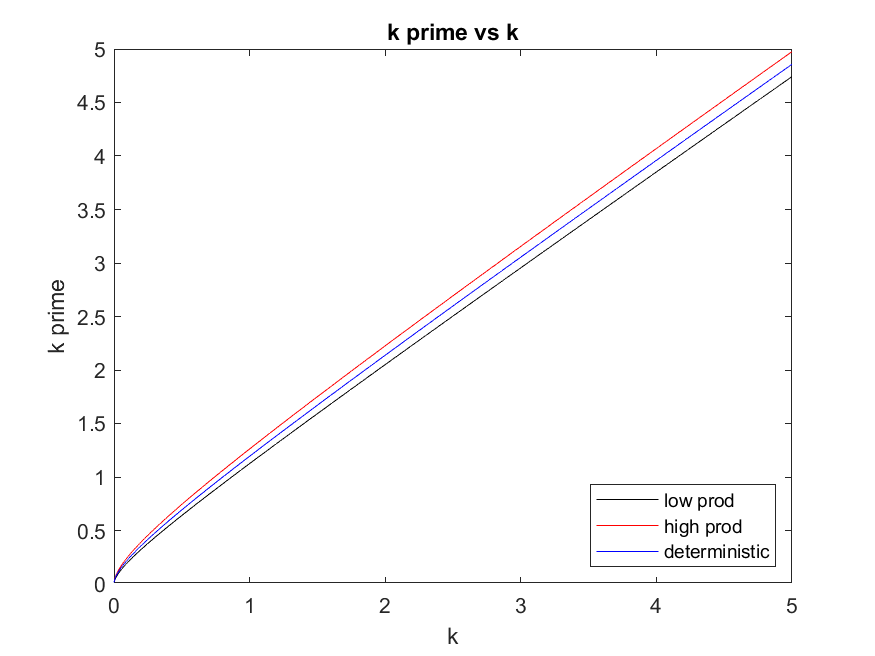
\includegraphics{q2k}

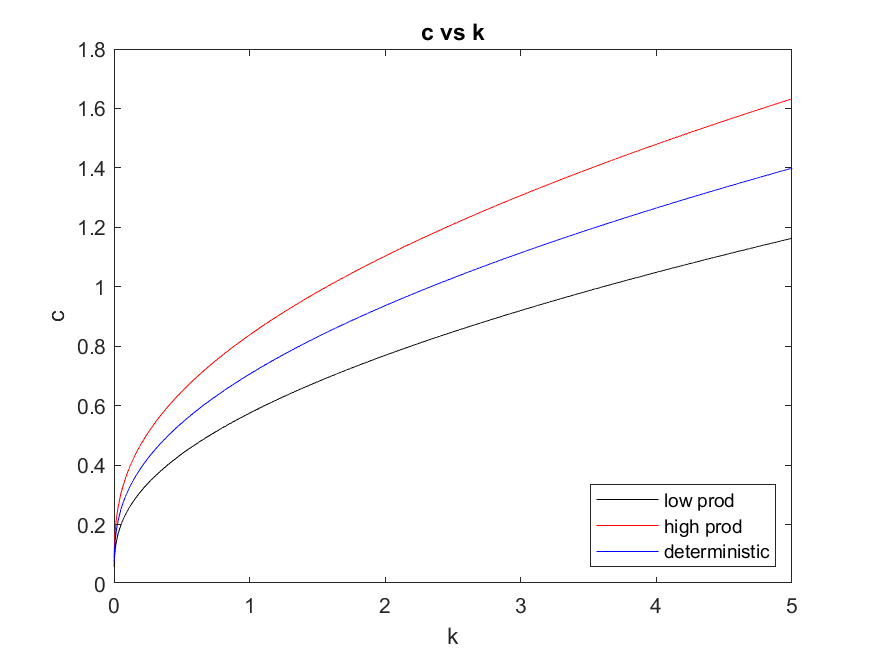
\includegraphics{q2c}

The above plots show that the consumption levels of the high and low equilibrium are, as expected, above and below the original equilibrium. A similar story holds for capital.

\subsection{Part B}
We start with an initial distribution of capital levels and, after a burn-in period, track capital, output, consumption, investment, wages, and interest rates over time. I ran the simulation 10000 times with a burn-in of 1000 draws (for a total of 11000 draws) from an initial uniform distribution over the states, and the averages of the variables of interest appeared to converge by the end of the simulation period. Results and comparison to the deterministic model are below.

\begin{center}
\begin{tabular}{lll}
& Deterministic & Simulation \\ 
\hline 
Capital & 3.5841 & 3.6302 \\ 
Output & 1.5633 & 1.5653 \\ 
Consumption & 1.2049 & 1.2182 \\ 
Investment & 0.35841 & 0.36302 \\ 
wages & 1.0161 & 1.0174 \\ 
interest rates & 0.15266 & 0.15373 \\ 
\hline 
\end{tabular}
\end{center}

On average, consumption in the stochastic case is higher than the deterministic case. This is due to capital being higher on average in the stochastic case compared to the deterministic case. Individuals are saving more to hedge against the bad productivity draws that may come in the future, and therefore end up consuming more on average as they are wealthier on average.

\subsection{Part C}
We calculate the volatilities and correlations as requested, reported below.

\begin{center}
\begin{tabular}{ll}
& Simulation \\ 
\hline 
Consumption Volatility & 0.26209 \\ 
Output Volatility & 0.092208 \\ 
Investment Volatility & 0.10719 \\ 
C-Y Correlation & 0.71852 \\ 
r-Y Correlation & -0.99692 \\ 
\hline 
\end{tabular}
\end{center}

We can see that consumption's volatility is high, much higher than output or investment volatility (reported volatility measures are the standard deviations of the simulated time series). Output and investment volatilities are roughly similar.

We see a high and positive correlation between output and consumption. This makes sense as more output implies a higher budget, and therefore higher consumption. The near-perfect negative correlation between the interest rate and output is very interesting. In this model, this is caused by the fact that both the interest rate and output are exactly determined by the capital level, so for small changes in capital levels the relationships between both the interest rate and output with capital levels are approximately linear, and therefore there is an approximate linear mapping between the interest rate and output (i.e. first-order taylor approximations mapping capital to the interest rate and capital to output yield a linear mapping between the interest rate and output). The near-unit magnitude of the correlation implies that the capital level is fluctuating by a sufficiently small amount over time for the approximate linear mappings between these variables to be very accurate.

\end{document}
